\chapter{Resultados de la red convolucional}
\label{cap:resultados}

Este capítulo presenta los resultados del protocolo de la Sección~\ref{sec:diseno}, en el orden en que se hicieron:
búsqueda de la tasa de aprendizaje, comparativa de los seis optimizadores con cinco semillas, evaluación clínica del
modelo elegido y comparación con los modelos convexos. En el medio aparece un resultado que no estaba previsto:
\emph{el paciente de validación no sirve para elegir}. Por eso se agregan dos análisis \emph{a posteriori} (el análisis
por crisis y el experimento con la tasa alta), que miran el conjunto de prueba y se informan como exploratorios.

En todo el capítulo, ``AUC de prueba'' es el AUC por ventana sobre chb03 y chb10 (201 ventanas ictales y 78\,998 sin
crisis, sin las de borde), y ``AUC de validación'' es el de chb01.

\section{Búsqueda de la tasa de aprendizaje}
\label{sec:res_busqueda}

La Tabla~\ref{tab:busqueda} muestra el resultado de las 18 corridas con semilla 0. La regla de elección es la de la
Sección~\ref{sec:diseno}: la tasa con mayor AUC de validación. La columna de prueba se agrega solo para el análisis
posterior; no intervino en la elección.

\begin{table}[ht]
\centering
\caption{Búsqueda de tasa de aprendizaje (semilla 0, 30 épocas). AUC de validación: mejor época, sobre el subconjunto
fijo de chb01. En negrita, la tasa elegida por validación. La columna de prueba se informa \emph{a posteriori}.}
\label{tab:busqueda}
\begin{tabular}{lcccc}
\toprule
Optimizador & $\eta$ & Paso efectivo & AUC validación & AUC prueba \\
\midrule
\multirow{3}{*}{SGD}
 & 0,03 & 0,03 & 0,9987 & 0,9355 \\
 & 0,1  & 0,1  & 0,9990 & 0,9480 \\
 & \textbf{0,3} & 0,3 & \textbf{0,9992} & 0,9802 \\
\midrule
\multirow{3}{*}{Momentum}
 & 0,003 & 0,03 & 0,9991 & 0,9049 \\
 & \textbf{0,01} & 0,1 & \textbf{0,9992} & 0,9121 \\
 & 0,03  & 0,3  & 0,9981 & 0,9592 \\
\midrule
\multirow{3}{*}{Nesterov}
 & \textbf{0,003} & 0,03 & \textbf{0,9990} & 0,8543 \\
 & 0,01  & 0,1  & 0,9981 & 0,8861 \\
 & 0,03  & 0,3  & 0,9988 & 0,9622 \\
\midrule
\multirow{3}{*}{RMSprop}
 & $\mathbf{3\times10^{-4}}$ & & \textbf{0,9983} & 0,9263 \\
 & $10^{-3}$        & & 0,9980 & 0,9794 \\
 & $3\times10^{-3}$ & & 0,9977 & 0,9704 \\
\midrule
\multirow{3}{*}{Adam}
 & $\mathbf{3\times10^{-4}}$ & & \textbf{0,9994} & 0,8707 \\
 & $10^{-3}$        & & 0,9983 & 0,9204 \\
 & $3\times10^{-3}$ & & 0,9987 & 0,9775 \\
\midrule
\multirow{3}{*}{AdamW}
 & $\mathbf{3\times10^{-4}}$ & & \textbf{0,9994} & 0,8728 \\
 & $10^{-3}$        & & 0,9983 & 0,8635 \\
 & $3\times10^{-3}$ & & 0,9975 & 0,9619 \\
\bottomrule
\end{tabular}
\end{table}

Lo primero que salta a la vista es que \textbf{las 18 corridas tienen un AUC de validación entre 0,9975 y 0,9994}: las
diferencias están en la cuarta cifra decimal. La elección se hizo igual, siguiendo el protocolo, pero sobre diferencias que,
como se verá en la Sección~\ref{sec:res_validacion}, son del orden del ruido entre semillas. Las tasas elegidas fueron
la más alta de la grilla para SGD, la del medio para Momentum y la más chica para Nesterov, RMSprop, Adam y AdamW.

\begin{figure}[ht]
  \centering
  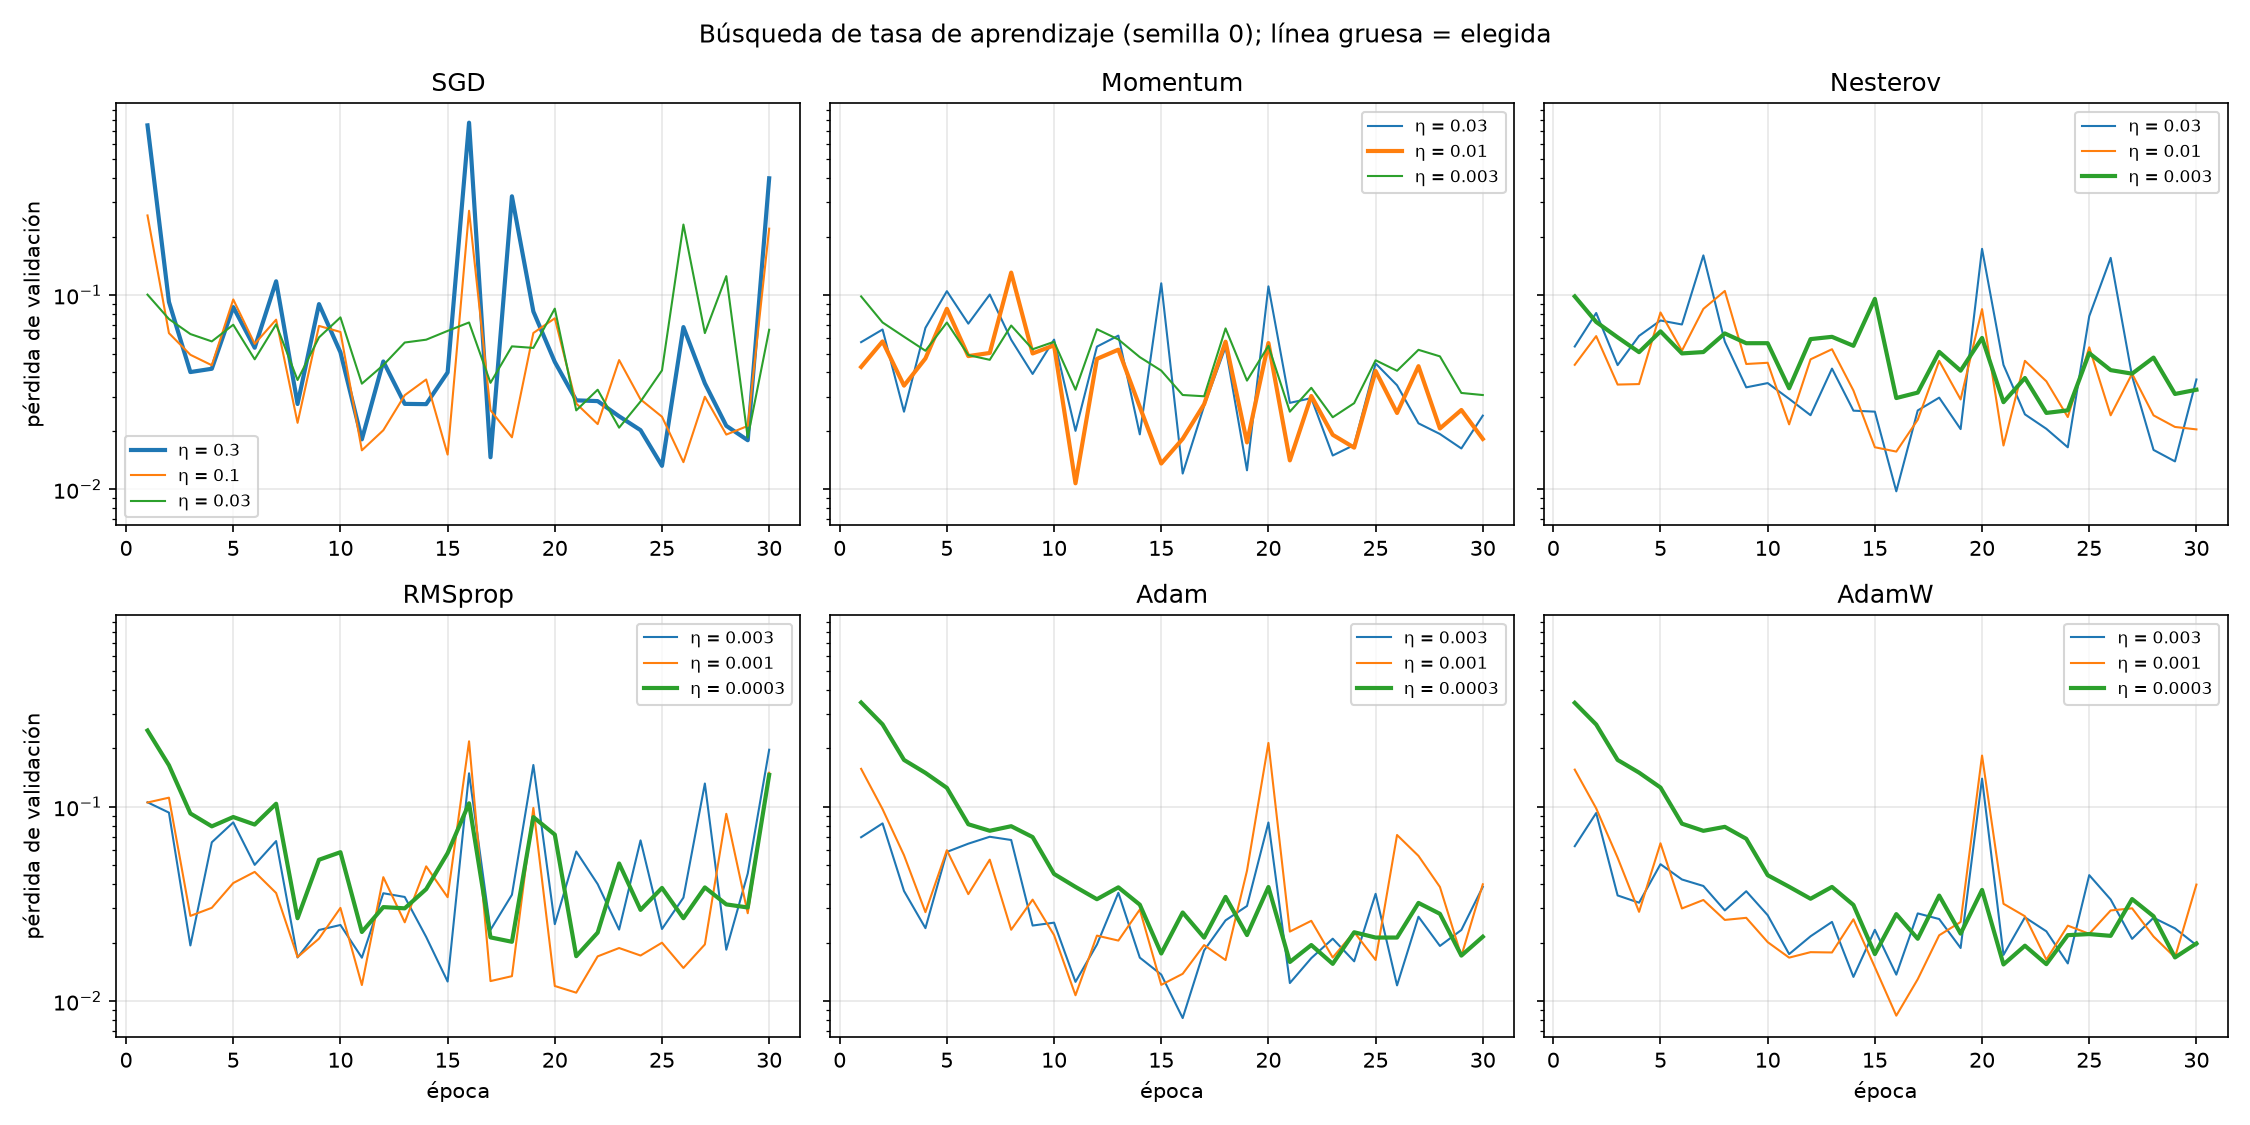
\includegraphics[width=\textwidth]{etapa4/busqueda_lr_curvas.png}
  \caption{Pérdida de validación (chb01) por época en la búsqueda de tasa, semilla 0. La línea gruesa es la tasa elegida.}
  \label{fig:busqueda_curvas}
\end{figure}

Las curvas de pérdida de validación (Figura~\ref{fig:busqueda_curvas}) muestran dos comportamientos. Con las tasas chicas de
los adaptativos ($3\times10^{-4}$) la pérdida baja de forma suave y lenta durante las primeras 10--15 épocas. Con las tasas
grandes, y sobre todo con SGD a $\eta = 0{,}3$, la pérdida salta de una época a otra en un orden de magnitud: hay épocas en las
que la red se desacomoda y se recupera en la siguiente. Es la señal de que el paso está cerca del límite de estabilidad del
lema de descenso (Sección~\ref{sec:gradiente}): en alguna dirección de curvatura alta, $\eta a$ se acerca o supera 2.

\section{Comparativa de optimizadores con cinco semillas}
\label{sec:res_comparativa}

\subsection{Resultado principal}

\begin{table}[ht]
\centering
\caption{Comparativa de optimizadores, cada uno con su tasa elegida por validación y 5 semillas. AUC de prueba: media $\pm$
desvío y rango. Época: mediana de la mejor época. Valor $p$: test de Mann-Whitney bilateral contra SGD.}
\label{tab:comparativa}
\begin{tabular}{lccccccc}
\toprule
Optimizador & $\eta$ & AUC val. & AUC prueba & Mín.--máx. & Época & $U$ & $p$ \\
\midrule
SGD      & 0,3              & 0,9982 & $\mathbf{0{,}9758 \pm 0{,}0063}$ & 0,966--0,981 & 26 & --- & --- \\
Momentum & 0,01             & 0,9984 & $0{,}9191 \pm 0{,}0341$ & 0,875--0,957 & 16 & 25 & 0,0079 \\
Nesterov & 0,003            & 0,9980 & $0{,}9196 \pm 0{,}0388$ & 0,854--0,957 & 24 & 25 & 0,0079 \\
RMSprop  & $3\times10^{-4}$ & 0,9982 & $0{,}9562 \pm 0{,}0224$ & 0,926--0,978 & 11 & 21 & 0,0952 \\
Adam     & $3\times10^{-4}$ & 0,9986 & $0{,}9171 \pm 0{,}0278$ & 0,871--0,939 & 16 & 25 & 0,0079 \\
AdamW    & $3\times10^{-4}$ & 0,9986 & $0{,}9225 \pm 0{,}0330$ & 0,873--0,960 & 16 & 25 & 0,0079 \\
\bottomrule
\end{tabular}
\end{table}

\begin{figure}[ht]
  \centering
  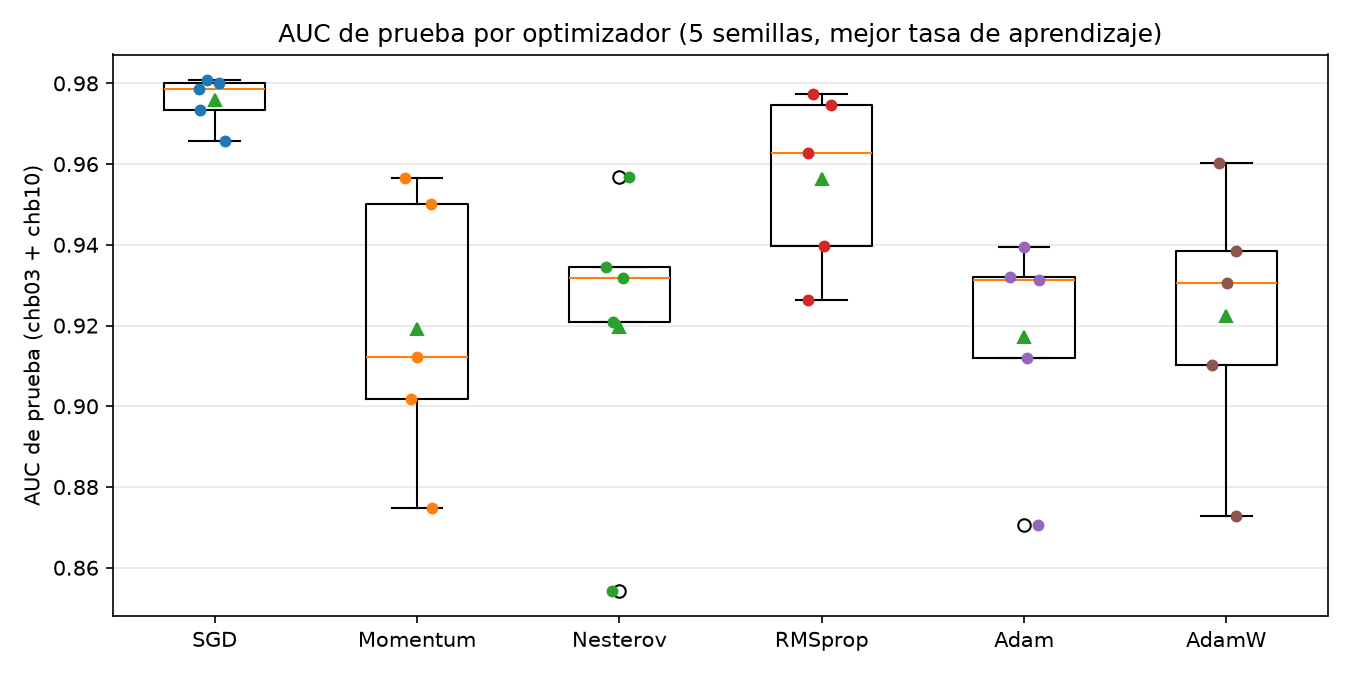
\includegraphics[width=0.9\textwidth]{etapa4/auc_prueba_por_optimizador.png}
  \caption{AUC de prueba de las 5 semillas de cada optimizador con su tasa elegida. Caja: cuartiles; línea naranja:
           mediana; triángulo: media.}
  \label{fig:auc_por_optimizador}
\end{figure}

Según la Tabla~\ref{tab:comparativa} y la Figura~\ref{fig:auc_por_optimizador}:
\begin{itemize}
  \item \textbf{SGD con $\eta = 0{,}3$ es el mejor y el más estable}: $0{,}976 \pm 0{,}006$. Su peor semilla (0,966) supera a
        la mejor de Adam (0,939).
  \item Contra Momentum, Nesterov, Adam y AdamW, las 5 semillas de SGD superan a las 5 del otro optimizador: $U = 25$,
        el máximo posible, con $p = 0{,}0079$. Es menor que el umbral de Bonferroni para 5 comparaciones ($0{,}01$), así que
        la diferencia se mantiene después de corregir.
  \item Contra RMSprop la diferencia no es significativa ($U = 21$, $p = 0{,}095$): RMSprop es el segundo, con mayor
        dispersión.
  \item Los otros cuatro quedan entre 0,917 y 0,923 de media, con desvíos de 0,03 a 0,04: la semilla mueve el resultado
        tanto como el optimizador.
  \item \textbf{El AUC de validación es prácticamente el mismo para los seis} (0,9980 a 0,9986), y ni siquiera ordena bien:
        Adam y AdamW tienen el mayor AUC de validación y están entre los peores en prueba.
\end{itemize}

Tomada al pie de la letra, la tabla coincidiría con \textcite{wilson2017}: el SGD simple generaliza mejor que los métodos
adaptativos. Pero la comparación es entre \emph{pares (optimizador, tasa)}, y la tasa la eligió un criterio que no
discrimina. Las secciones siguientes muestran que esa lectura no se sostiene.

\subsection{Curvas de entrenamiento}

\begin{figure}[ht]
  \centering
  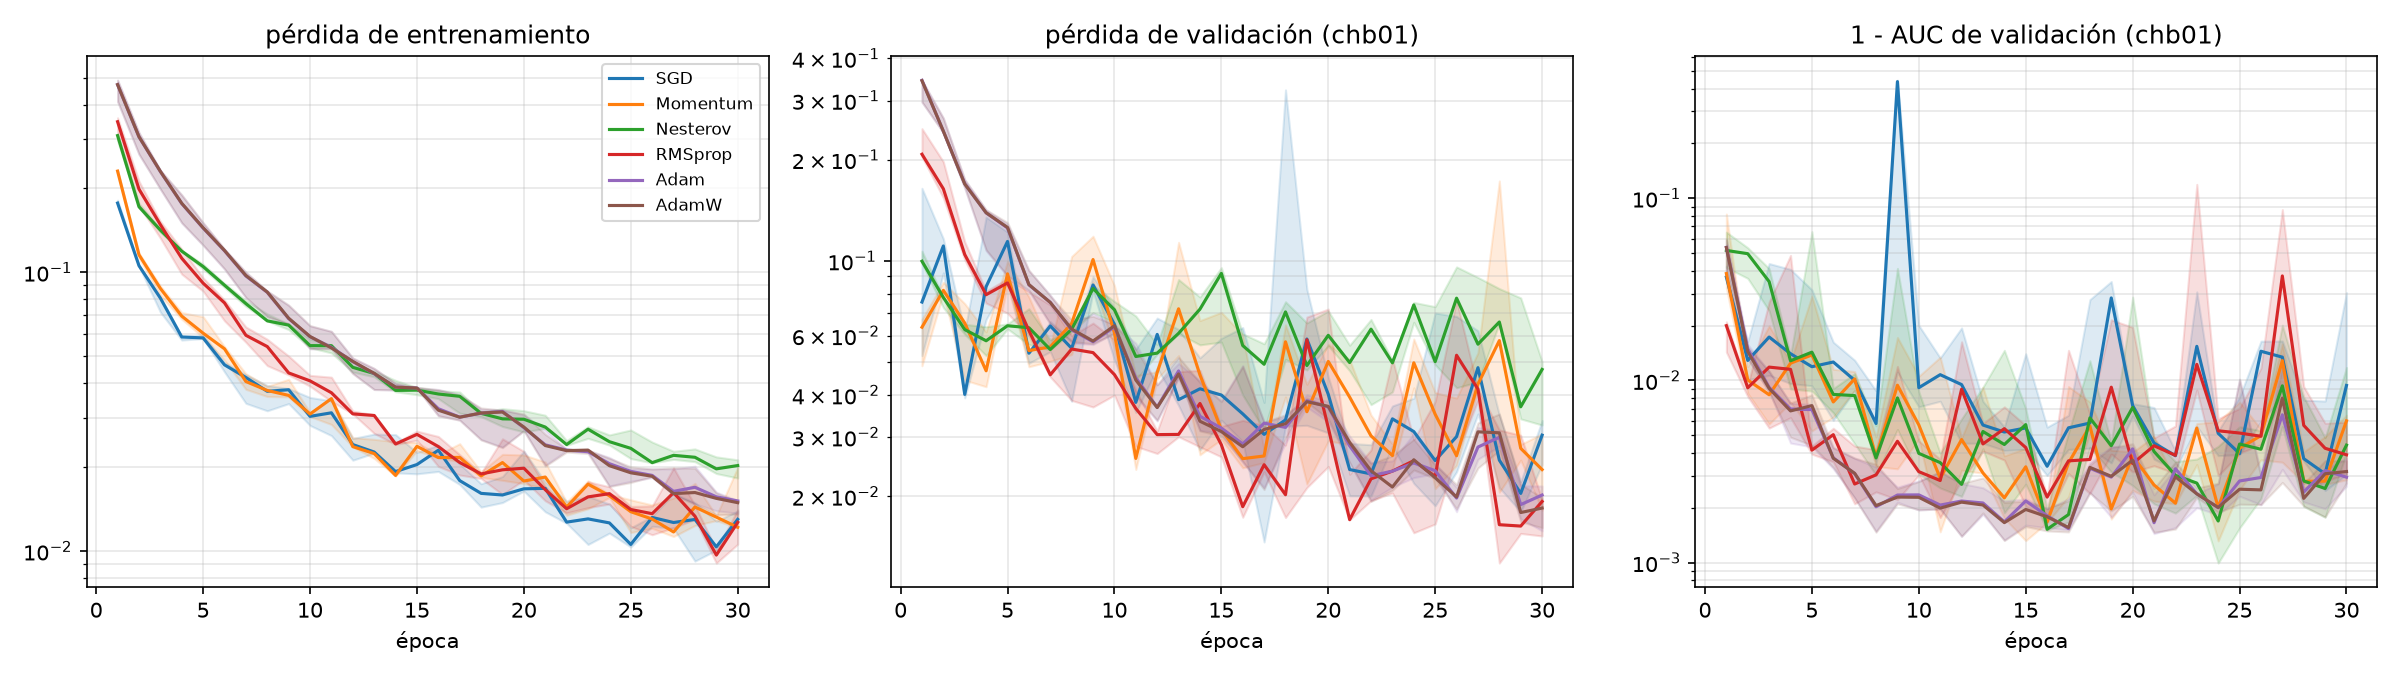
\includegraphics[width=\textwidth]{etapa4/curvas_optimizadores.png}
  \caption{Curvas de entrenamiento con la tasa elegida: mediana (línea) y rango intercuartil (sombra) sobre las 5 semillas.
           El AUC de validación se muestra como $1 - \text{AUC}$ en escala logarítmica.}
  \label{fig:curvas_optimizadores}
\end{figure}

La Figura~\ref{fig:curvas_optimizadores} muestra la evolución de las 30 épocas:
\begin{itemize}
  \item \textbf{Pérdida de entrenamiento.} SGD y Momentum bajan más rápido y terminan más abajo; Nesterov, Adam y AdamW
        quedan más arriba durante todo el entrenamiento. No es una propiedad de los algoritmos: son justamente los tres a los
        que la búsqueda les asignó la tasa más chica de su grilla. Con paso chico, en 2100 pasos la red no llega a ajustar
        tanto.
  \item \textbf{Inestabilidad de SGD.} Con $\eta = 0{,}3$, las 5 semillas tienen épocas en las que el AUC de validación cae
        de golpe por debajo de 0,7 (el mínimo es 0,21) y se recupera en la época siguiente; en la mediana se ve como el pico
        de la época 9. Momentum, con el mismo paso efectivo (0,3) en el experimento de la Sección~\ref{sec:res_tasa_alta}, no
        cae nunca por debajo de 0,81. Es lo que predice la Proposición~\ref{prop:momentum}: a igual paso efectivo, el momento
        amplía la región de estabilidad de $\eta_\text{ef}\,a < 2$ a $\eta_\text{ef}\,a < 38$. Guardar la mejor época evita
        que esas caídas afecten el resultado final.
  \item \textbf{Validación saturada.} Desde la época 8, todos los optimizadores quedan con $1 - \text{AUC}$ entre
        $2\times10^{-3}$ y $10^{-2}$ en validación (mediana de las semillas), con oscilaciones de época a época mayores que las diferencias entre optimizadores. La pérdida de
        validación, en cambio, sigue bajando lentamente: la red mejora la confianza de sus predicciones en chb01, pero el
        orden de los puntajes ya no cambia.
  \item \textbf{Mejor época.} RMSprop alcanza su mejor época antes (mediana 11) y SGD, más tarde (26). Con validación
        saturada, cuál época queda como ``mejor'' es en buena parte azar.
\end{itemize}

\section{La validación con un solo paciente no discrimina}
\label{sec:res_validacion}

\begin{figure}[ht]
  \centering
  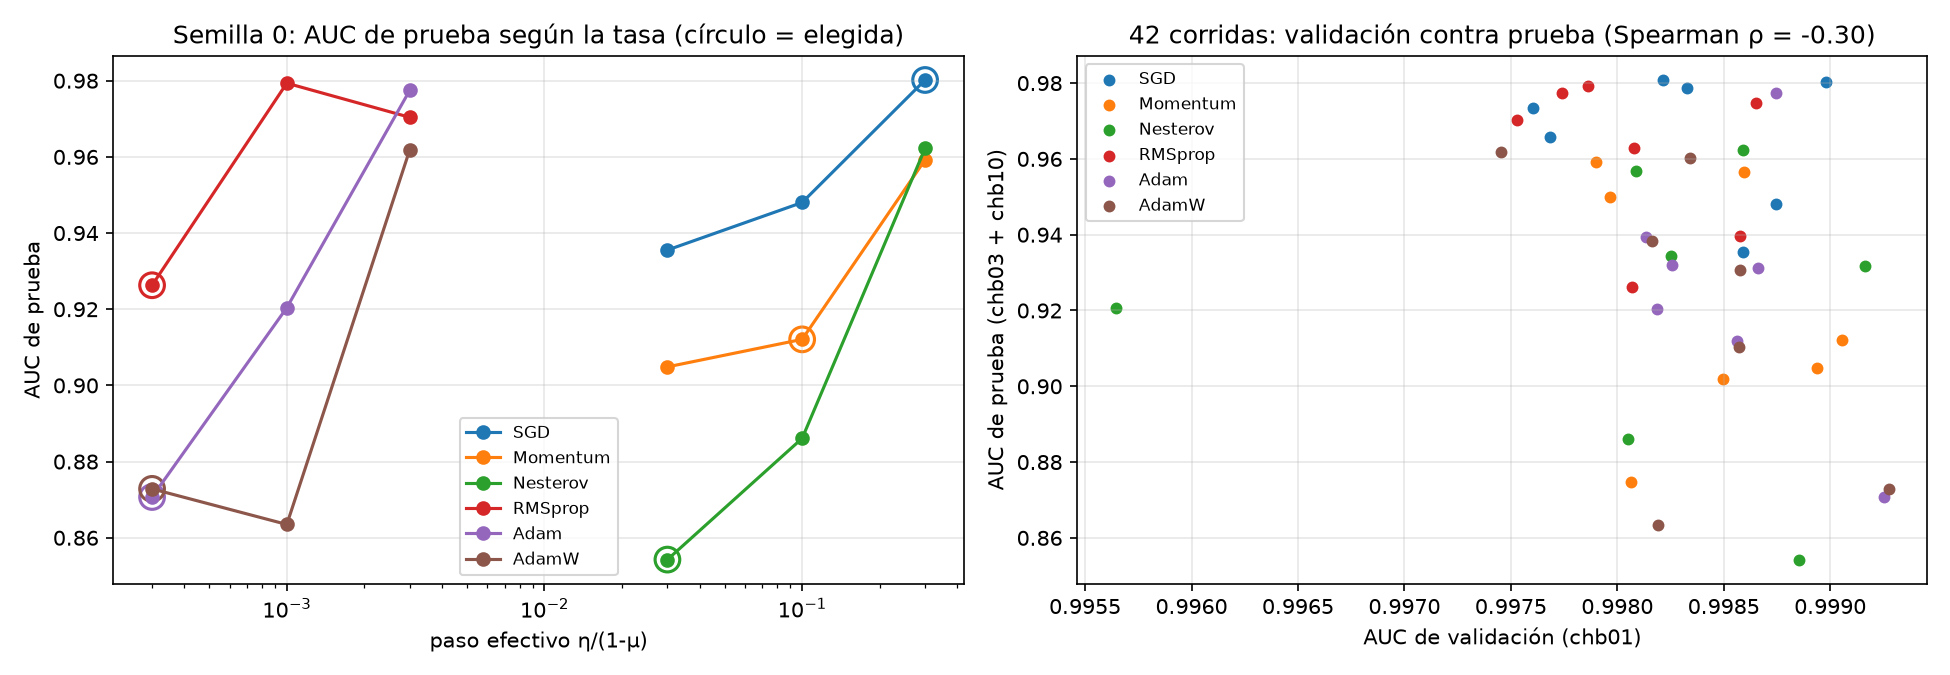
\includegraphics[width=\textwidth]{etapa4/validacion_vs_prueba.png}
  \caption{Izquierda: AUC de prueba de la semilla 0 en función del paso efectivo; el círculo marca la tasa elegida por
           validación. Derecha: AUC de validación contra AUC de prueba en las 42 corridas del diseño original.}
  \label{fig:validacion_vs_prueba}
\end{figure}

La Figura~\ref{fig:validacion_vs_prueba} resume el problema.
\begin{itemize}
  \item \textbf{Rangos.} En las 42 corridas, el AUC de validación (sobre las 36\,496 ventanas de chb01) varía entre 0,9956 y
        0,9993, y el de prueba, entre 0,854 y 0,981. La validación cambia en milésimas y la prueba, en décimas.
  \item \textbf{Correlación.} La correlación de Spearman entre ambos es $\rho = -0{,}30$ ($p = 0{,}06$). No solo no hay
        asociación positiva: la tendencia, no significativa, es la contraria. Las corridas con mayor AUC de validación
        (por encima de 0,999) incluyen algunas de las peores en prueba.
  \item \textbf{La tasa elegida.} En la semilla 0, la tasa \emph{más alta} de la grilla dio el mejor AUC de prueba en cinco
        de los seis optimizadores (en RMSprop, la del medio). La validación eligió esa tasa solo para SGD. Para Nesterov,
        Adam y AdamW eligió la que en prueba resultó peor o casi peor.
\end{itemize}

¿Por qué pasa esto? chb01 es un paciente ``fácil'': todas las redes, desde la época 8, separan sus crisis casi
perfectamente. Un conjunto de validación en el que todos los modelos aciertan no puede ordenarlos. Las diferencias entre
corridas aparecen en otro lado: en lo que la red hace con un paciente cuyas crisis son distintas de las que vio. La
Sección~\ref{sec:res_percentil} muestra exactamente dónde.

Desde el punto de vista del diseño, la lección es clara: \textbf{un solo paciente de validación no alcanza para elegir
hiperparámetros} en un problema donde lo que se busca es generalizar entre pacientes. Habría hecho falta validación
cruzada por paciente también para la búsqueda de tasa, como el LOPO del Capítulo~\ref{cap:convexos}, aunque eso
multiplica el costo de entrenamiento.

\section{Análisis por crisis}
\label{sec:res_percentil}

Para entender de dónde salen las diferencias en el AUC de prueba se calcula, para cada corrida y cada una de las 14 crisis
de prueba, el \textbf{percentil} del puntaje mediano de las ventanas de la crisis dentro de la distribución de las 78\,998
ventanas sin crisis de prueba. Un percentil de 1 significa que la crisis está por encima de todas las ventanas normales; uno
de 0,5, que no se distingue de ellas; uno cercano a 0, que la red la puntúa \emph{más bajo} que casi cualquier ventana normal.
Como el AUC es el promedio, sobre las ventanas ictales, de la fracción de negativos que cada una supera
(Proposición~\ref{prop:auc}), este percentil es su versión por crisis.

\begin{figure}[ht]
  \centering
  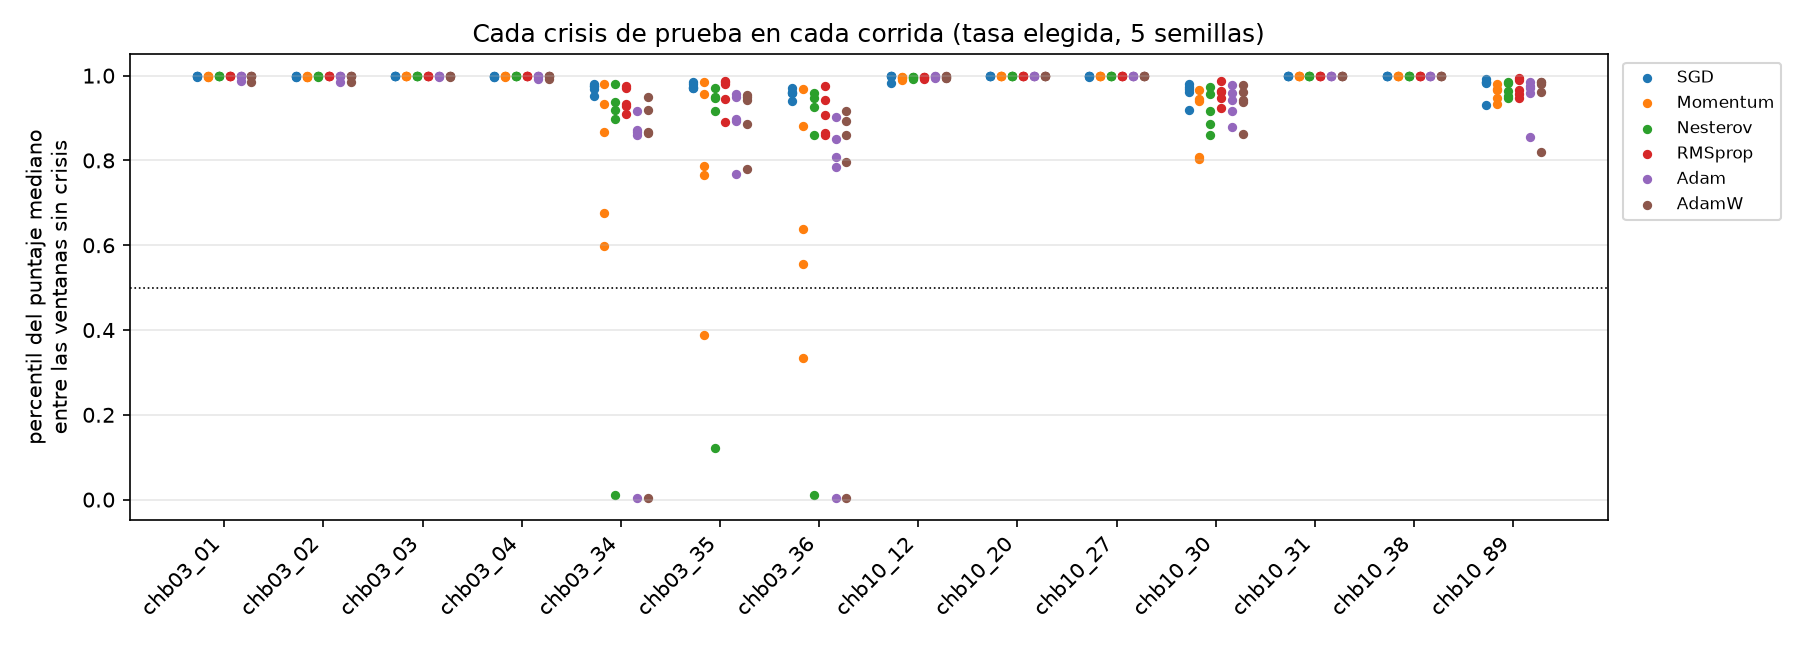
\includegraphics[width=\textwidth]{etapa4/percentil_por_crisis.png}
  \caption{Percentil del puntaje mediano de cada crisis de prueba entre las ventanas sin crisis, para las 30 corridas con la
           tasa elegida (5 semillas por optimizador). La línea punteada es 0,5 (indistinguible del azar).}
  \label{fig:percentil_crisis}
\end{figure}

\begin{table}[ht]
\centering
\caption{Percentil medio de las tres crisis difíciles de chb03 por optimizador (tasa elegida, 5 semillas). Las otras 11
crisis tienen percentil medio de 0,93 o más.}
\label{tab:percentil_opt}
\begin{tabular}{lccc}
\toprule
Optimizador & chb03\_34 & chb03\_35 & chb03\_36 \\
\midrule
SGD      & 0,971 & 0,976 & 0,958 \\
RMSprop  & 0,944 & 0,958 & 0,910 \\
Momentum & 0,811 & 0,777 & 0,676 \\
Nesterov & 0,749 & 0,782 & 0,741 \\
Adam     & 0,704 & 0,893 & 0,670 \\
AdamW    & 0,721 & 0,902 & 0,694 \\
\bottomrule
\end{tabular}
\end{table}

Los resultados (Figura~\ref{fig:percentil_crisis} y Tabla~\ref{tab:percentil_opt}) son muy concentrados:
\begin{itemize}
  \item \textbf{11 de las 14 crisis las reconocen bien todas las corridas.} Las cuatro primeras de chb03 y las siete de chb10
        tienen percentil medio entre 0,93 y 1, con desvío entre corridas menor a 0,05.
  \item \textbf{Toda la variabilidad está en tres crisis de un mismo paciente}: chb03\_34, chb03\_35 y chb03\_36, de los
        registros del final de la internación. Su desvío entre corridas es de 0,2 a 0,3. En algunas corridas, entre ellas el
        modelo final (AdamW, semilla 0) y Adam con semilla 0, dos de ellas quedan con percentil 0,004: \emph{por debajo del 99,6~\% de las ventanas
        normales}.
  \item El percentil medio de esas tres crisis explica el ranking de prueba: su correlación de Spearman con el AUC de prueba,
        sobre las 42 corridas, es $\rho = 0{,}87$ ($p < 10^{-13}$).
  \item La Tabla~\ref{tab:percentil_opt} reproduce la separación de la Tabla~\ref{tab:comparativa}: SGD y RMSprop
        puntúan alto esas tres crisis en todas sus semillas; los otros cuatro, con la tasa elegida, no siempre.
\end{itemize}

La consecuencia para la comparativa es importante: \textbf{el conjunto de prueba efectivo para distinguir optimizadores son
tres crisis de un paciente}. Todas las conclusiones sobre qué optimizador es mejor dependen de qué pasa con ellas, y no se
pueden generalizar mucho más allá de este caso.

\section{Experimento de sensibilidad: todos con la tasa alta}
\label{sec:res_tasa_alta}

La búsqueda sugería que la ventaja de SGD podía deberse a la tasa y no al algoritmo: a SGD la validación le dio la tasa
alta, y a los demás no. Para probarlo, se corrió cada optimizador con la tasa más alta de su grilla y 5 semillas. Este
experimento se diseñó \textbf{después de mirar la prueba}, así que es exploratorio: no cambia el modelo elegido ni las
conclusiones de las Secciones~\ref{sec:res_comparativa} y~\ref{sec:res_clinica}, y sus valores $p$ no tienen la
interpretación de un test planificado.

\begin{table}[ht]
\centering
\caption{Experimento exploratorio: cada optimizador con la tasa más alta de su grilla, 5 semillas. Se repite la media con la
tasa elegida para comparar. Valor $p$: Mann-Whitney bilateral contra SGD.}
\label{tab:tasa_alta}
\begin{tabular}{lcccccc}
\toprule
 & & \multicolumn{3}{c}{Tasa alta} & Tasa elegida & \\
\cmidrule(lr){3-5}\cmidrule(lr){6-6}
Optimizador & $\eta$ & AUC val. & AUC prueba & Mín. & AUC prueba & $p$ \\
\midrule
SGD      & 0,3              & 0,9982 & $0{,}9758 \pm 0{,}0063$ & 0,966 & 0,9758 & --- \\
Momentum & 0,03             & 0,9979 & $0{,}9596 \pm 0{,}0067$ & 0,950 & 0,9191 & 0,016 \\
Nesterov & 0,03             & 0,9987 & $0{,}9501 \pm 0{,}0285$ & 0,905 & 0,9196 & 0,056 \\
RMSprop  & $3\times10^{-3}$ & 0,9976 & $0{,}9730 \pm 0{,}0132$ & 0,952 & 0,9562 & 1,000 \\
Adam     & $3\times10^{-3}$ & 0,9984 & $0{,}9712 \pm 0{,}0091$ & 0,957 & 0,9171 & 0,310 \\
AdamW    & $3\times10^{-3}$ & 0,9975 & $0{,}9699 \pm 0{,}0076$ & 0,962 & 0,9225 & 0,222 \\
\bottomrule
\end{tabular}
\end{table}

\begin{figure}[ht]
  \centering
  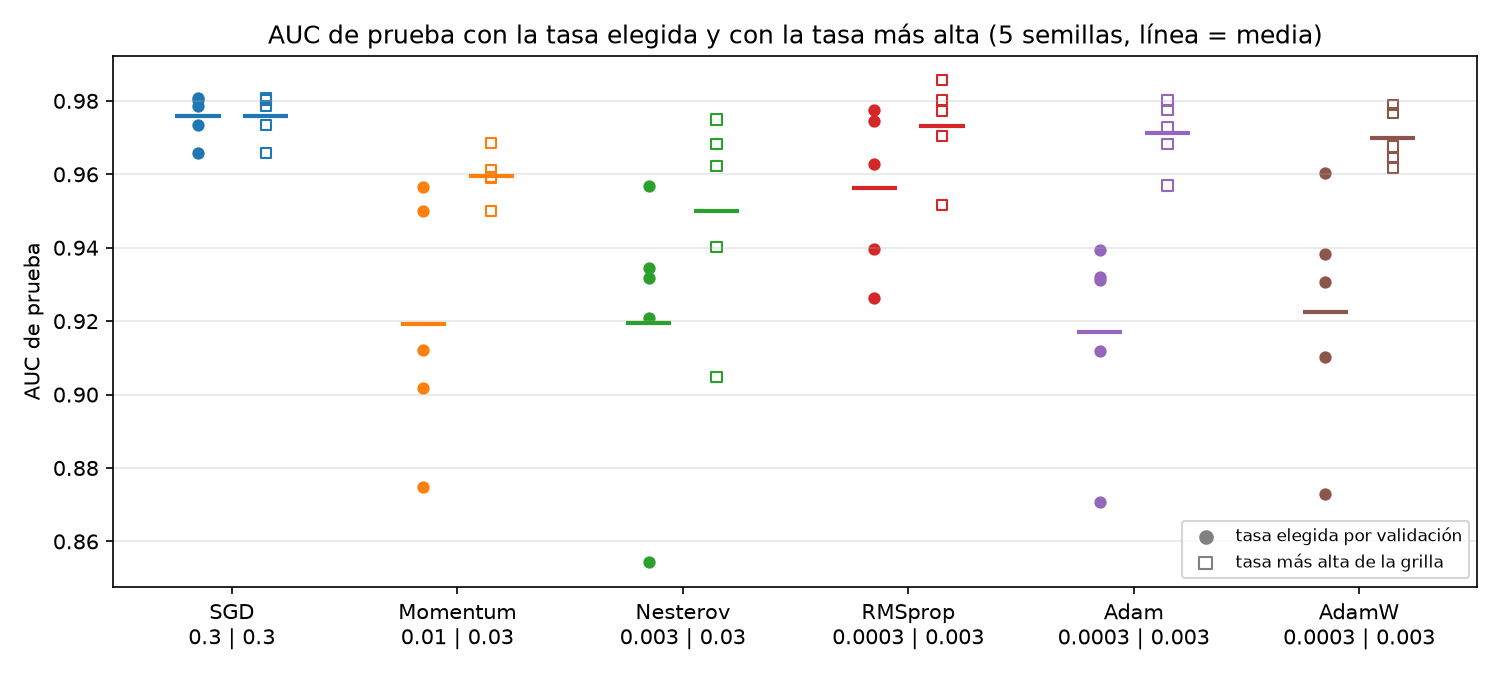
\includegraphics[width=\textwidth]{etapa4/tasa_elegida_vs_alta.png}
  \caption{AUC de prueba de las 5 semillas de cada optimizador con la tasa elegida por validación (círculos) y con la tasa
           más alta de la grilla (cuadrados). La línea horizontal es la media.}
  \label{fig:tasa_alta}
\end{figure}

La Tabla~\ref{tab:tasa_alta} y la Figura~\ref{fig:tasa_alta} confirman la hipótesis:
\begin{itemize}
  \item \textbf{Con la tasa alta, todos mejoran} y la dispersión baja mucho. Adam pasa de $0{,}917 \pm 0{,}028$ a
        $0{,}971 \pm 0{,}009$; AdamW, de $0{,}923 \pm 0{,}033$ a $0{,}970 \pm 0{,}008$.
  \item \textbf{RMSprop, Adam y AdamW quedan empatados con SGD}: medias entre 0,970 y 0,976, y valores $p$ entre 0,22 y 1.
        La ``ventaja de SGD sobre los adaptativos'' de la Tabla~\ref{tab:comparativa} era, sobre todo, una ventaja de la tasa.
  \item \textbf{Momentum} queda algo por debajo (0,960) con el mismo paso efectivo que SGD. La diferencia es consistente
        (SGD gana en 24 de los 25 pares de semillas, $U = 24$, $p = 0{,}016$) pero no pasa la corrección de Bonferroni.
  \item \textbf{Nesterov} sigue siendo el más irregular: una semilla en 0,905 y desvío de 0,029.
  \item \textbf{La validación tampoco habría elegido estas tasas}: su AUC de validación medio (0,9975 a 0,9987) es igual o
        menor que el de las tasas elegidas. El problema no es la regla de elección sino que chb01 no discrimina.
\end{itemize}

\subsection{Interpretación}

¿Por qué la tasa alta generaliza mejor a chb03? No hay una demostración, pero hay tres elementos consistentes con lo
observado:
\begin{enumerate}
  \item \textbf{Ruido y mínimos planos.} Con paso grande, el ruido del gradiente estocástico impide que la red se acomode en
        regiones angostas de la pérdida, que tienden a depender de detalles de los tres pacientes de entrenamiento.
        Las caídas de validación de SGD con $\eta = 0{,}3$ muestran que el entrenamiento está, efectivamente, cerca del borde
        de la estabilidad.
  \item \textbf{Normalización por lotes.} Por la Proposición~\ref{prop:bn_escala}, la tasa efectiva de las capas convolucionales
        depende de $\eta/\lVert\vw\rVert^2$. Con tasa alta las normas crecen más rápido, y la dinámica cambia en formas que no se
        reducen a ``más paso''.
  \item \textbf{Menos ajuste a los pacientes de entrenamiento.} Con tasa chica, Adam y AdamW tienen la pérdida de
        entrenamiento más alta (Figura~\ref{fig:curvas_optimizadores}), pero aun así generalizan peor. No es un problema de
        sobreajuste clásico (más pérdida de entrenamiento con peor prueba), sino de \emph{qué} solución se encuentra entre
        muchas con pérdida parecida, que es lo esperable en una función no convexa (Sección~\ref{sec:no_convexo}).
\end{enumerate}

La conclusión de la comparativa, con la cautela que impone haber diseñado este experimento después de ver la prueba, es que
\textbf{en este problema el factor que más pesa en la generalización a pacientes nuevos es la tasa de aprendizaje, más que el
algoritmo}. Con la tasa adecuada, los seis optimizadores quedan entre 0,95 y 0,98, y SGD, RMSprop, Adam y AdamW no se
distinguen con 5 semillas.

\section{Evaluación clínica del modelo elegido}
\label{sec:res_clinica}

\subsection{El modelo elegido}

El protocolo elige el optimizador con mayor AUC de validación medio y, dentro de él, la semilla con mayor AUC de validación.
Resulta \textbf{AdamW con $\eta = 3\times10^{-4}$, semilla 0} (AUC de validación 0,9993, mejor época 15). Adam y AdamW
empatan en 0,9986 de AUC de validación medio, y el desempate a la cuarta cifra favorece a AdamW.

Con lo visto en las secciones anteriores, es una mala elección: en prueba es una de las peores corridas (AUC 0,873). Se
informa igual. Cambiar el modelo después de mirar la prueba invalidaría la estimación de su desempeño, que es lo que el
conjunto de prueba debe dar. Es preferible informar un modelo peor con una estimación honesta que uno mejor con una
estimación sesgada.

\subsection{Métricas por ventana y por evento}

Se aplica el procedimiento de la Sección~\ref{sec:umbral_np}: suavizado causal de 3 ventanas y umbral de Neyman-Pearson con
$\alpha = 10^{-3}$ calculado con las ventanas sin crisis de chb01.

\begin{figure}[ht]
  \centering
  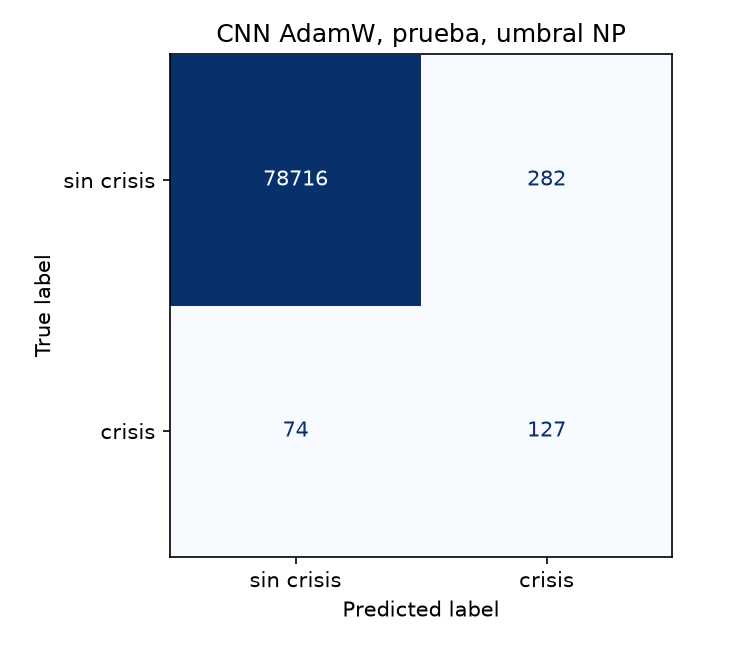
\includegraphics[width=0.5\textwidth]{etapa4/confusion_cnn.png}
  \caption{Matriz de confusión por ventana de la CNN final en prueba (chb03 y chb10, sin ventanas de borde), con umbral de
           Neyman-Pearson.}
  \label{fig:confusion_cnn}
\end{figure}

\begin{table}[ht]
\centering
\caption{CNN final (AdamW, semilla 0) en los pacientes de prueba, umbral de Neyman-Pearson con $\alpha = 10^{-3}$.}
\label{tab:cnn_pacientes}
\begin{tabular}{lccc}
\toprule
 & chb03 & chb10 & Total \\
\midrule
AUC                         & 0,726 & 0,995 & 0,872 \\
$TP$ / $FN$                 & 46 / 50 & 81 / 24 & 127 / 74 \\
$FP$ / $TN$                 & 242 / 33\,853 & 40 / 44\,863 & 282 / 78\,716 \\
Sensibilidad por ventana    & 0,479 & 0,771 & 0,632 \\
Especificidad por ventana   & 0,9929 & 0,9991 & 0,9964 \\
VPP por ventana             & 0,160 & 0,669 & 0,311 \\
Crisis detectadas           & 4/7 & 7/7 & 11/14 \\
Horas sin crisis            & 37,9 & 49,9 & 87,8 \\
Falsas alarmas              & 98 & 21 & 119 \\
Falsas alarmas por hora     & 2,59 & 0,42 & 1,36 \\
Latencia mediana [s]        & 9 & 11 & 11 \\
\bottomrule
\end{tabular}
\end{table}

La Tabla~\ref{tab:cnn_pacientes} y la Figura~\ref{fig:confusion_cnn} muestran dos pacientes muy distintos.
\begin{itemize}
  \item \textbf{chb10 sale casi perfecto}: AUC 0,995, las 7 crisis detectadas con una latencia mediana de 11~s y 0,42 falsas
        alarmas por hora (una cada dos horas y media).
  \item \textbf{chb03 es el paciente difícil}: AUC 0,73. Se detectan las 4 crisis de los registros chb03\_01 a chb03\_04, con
        latencias de 6 a 13~s, pero ninguna de las de chb03\_34 a chb03\_36. Además genera 2,6 falsas alarmas por hora.
\end{itemize}

Las crisis no detectadas no son ``débiles'': respecto del resto de su registro, tienen un aumento de potencia por banda
\emph{mayor} que las detectadas (del orden de 1,7 contra 1,2 en $\log_{10}$), y la regresión logística calibrada, que solo
mira la potencia por banda, les da puntajes altos. La red aprendió de los tres pacientes de entrenamiento un patrón
espectro-temporal más específico que ``sube la potencia'', y ese patrón no aparece en estas tres crisis. Es el precio de un
modelo más expresivo entrenado con 13 crisis.

\paragraph{La restricción de Neyman-Pearson en cada paciente.} Con $\alpha = 10^{-3}$ y 900 ventanas por hora se esperan
unas 0,9 ventanas falsas por hora. En chb10 hay $40/49{,}9 = 0{,}8$: la restricción se cumple. En chb03 hay
$242/37{,}9 = 6{,}4$, siete veces más. Es otra vez la Observación~\ref{obs:np_supuesto}: el umbral se calibró con la
distribución del puntaje de chb01, y la de chb03 tiene la cola derecha más pesada. Una calibración del umbral con un
período inicial del propio paciente lo corregiría en buena parte.

\paragraph{Valor predictivo.} De las 409 ventanas declaradas como crisis, 127 lo son: VPP de 0,31, como se anticipó con la
ecuación~\eqref{eq:vpp_bayes}. Por evento, las 282 ventanas falsas se agrupan en 119 alarmas.

\section{Comparación con los modelos convexos}
\label{sec:res_comparacion}

\begin{table}[ht]
\centering
\caption{Partición fija, prueba en chb03 y chb10 (14 crisis, 87,8 horas sin crisis). Suavizado de 3 ventanas y umbral de
Neyman-Pearson con $\alpha = 10^{-3}$ calibrado en chb01. ``Sens. a $10^{-3}$'': sensibilidad por ventana con una tasa de
falsos positivos de $10^{-3}$ en la propia prueba (leída de la curva ROC).}
\label{tab:comparacion_final}
\begin{tabular}{lccccccc}
\toprule
Modelo & AUC & Sens. a $10^{-3}$ & Sens. & Espec. & Crisis & FA/h & Lat. [s] \\
\midrule
Logística (global)     & 0,799 & 0,00 & 0,304 & 0,9849 & 5/14 & 3,26 & 14,0 \\
SVM lineal (global)    & 0,798 & 0,00 & 0,304 & 0,9865 & 7/14 & 2,94 & 18,0 \\
Logística (calibrada)  & \textbf{0,934} & 0,02 & 0,269 & 0,9941 & 7/14 & 1,22 & 26,0 \\
SVM lineal (calibrado) & 0,930 & 0,02 & 0,244 & 0,9946 & 6/14 & \textbf{1,00} & 24,5 \\
CNN AdamW              & 0,872 & \textbf{0,54} & \textbf{0,632} & \textbf{0,9964} & \textbf{11/14} & 1,36 & \textbf{11,0} \\
\bottomrule
\end{tabular}
\end{table}

\begin{figure}[ht]
  \centering
  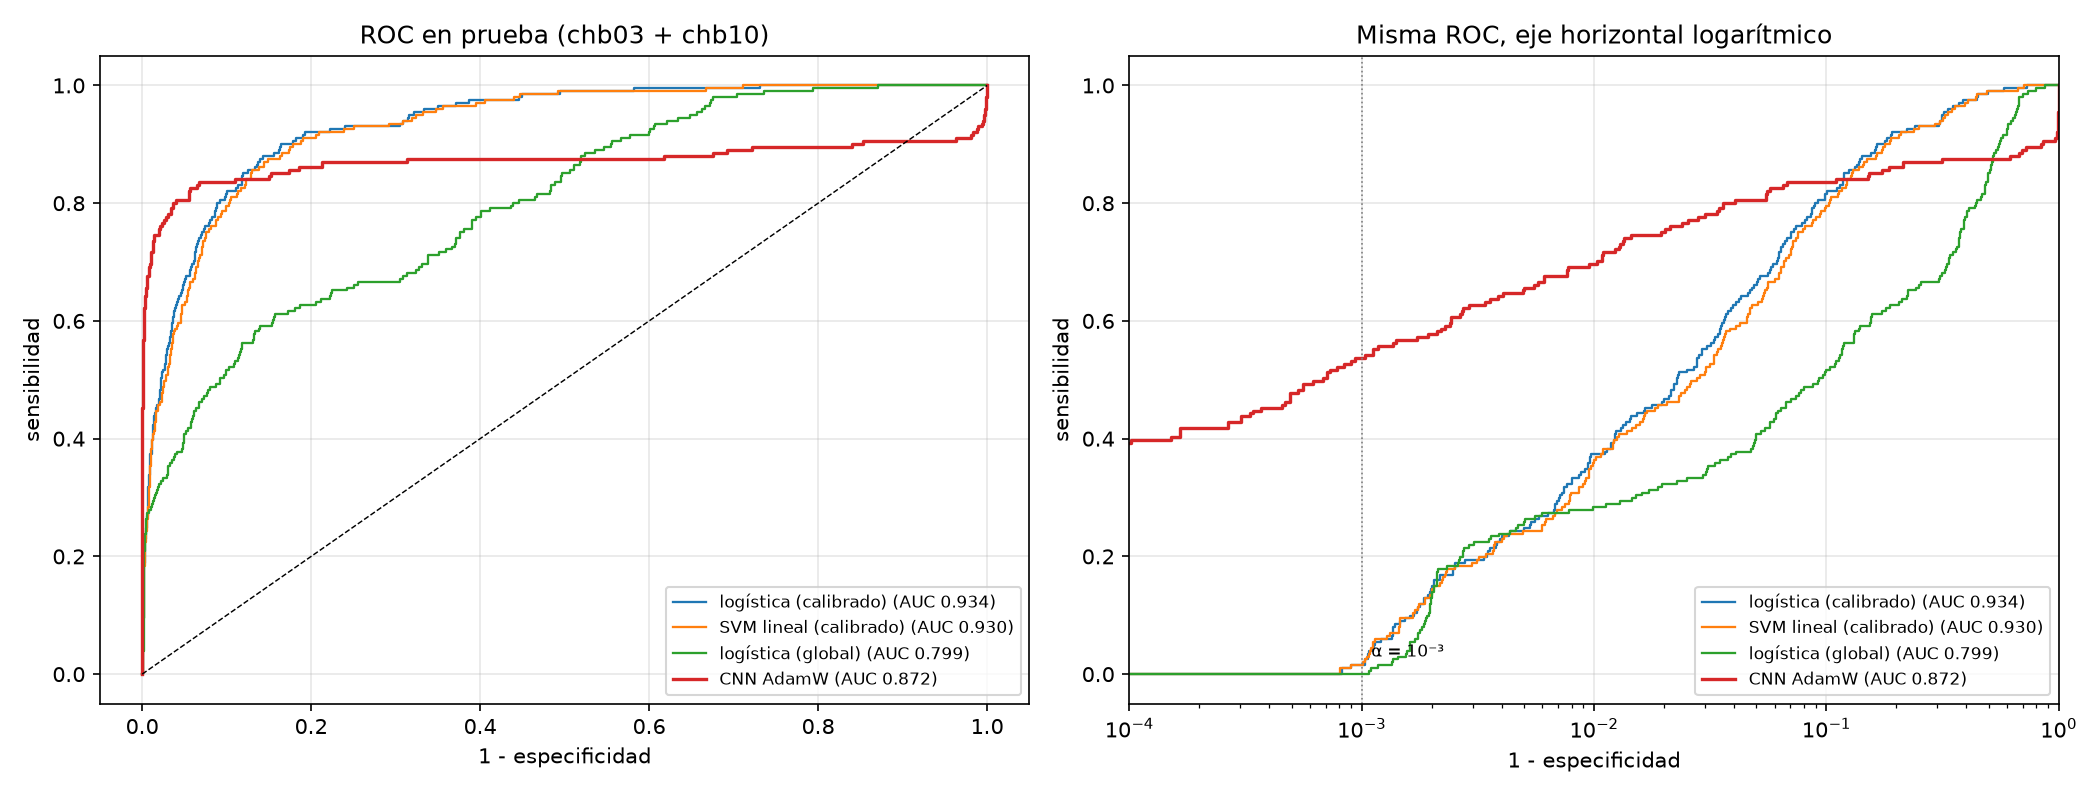
\includegraphics[width=\textwidth]{etapa4/roc_cnn_vs_convexos.png}
  \caption{Curvas ROC en prueba de la CNN final y de los modelos convexos. Izquierda: ejes lineales. Derecha: eje horizontal
           logarítmico; la línea punteada marca $\text{FPR} = 10^{-3}$.}
  \label{fig:roc_cnn}
\end{figure}

La Tabla~\ref{tab:comparacion_final} y la Figura~\ref{fig:roc_cnn} muestran el caso que se anticipó en la
Sección~\ref{sec:zona_util}: \textbf{el modelo con menor AUC es el mejor detector}.
\begin{itemize}
  \item En ejes lineales, la logística calibrada parece mejor: su curva está por encima de la de la CNN desde un 12~\% de
        falsos positivos, y su AUC es 0,934 contra 0,872.
  \item En escala logarítmica la situación se invierte. Con $\text{FPR} = 10^{-3}$ (0,9 ventanas falsas por hora), la CNN detecta
        el 54~\% de las ventanas ictales y la logística calibrada, el 2~\%: su curva recién despega a partir de $10^{-3}$. Con
        $\text{FPR} = 10^{-4}$ la CNN todavía detecta el 39~\% y la logística, ninguna. Con $\text{FPR} = 10^{-2}$: 70~\% contra 37~\%.
  \item La curva de la CNN casi \textbf{se estanca} desde un 10~\% de falsos positivos: pasa de 0,84 a solo 0,90 con 95~\% de
        falsos positivos, mientras la logística llega a 0,99 con 50~\%. Las ventanas de chb03\_34 a chb03\_36 tienen un puntaje
        menor que la mayoría de las ventanas normales. Ese tramo es el que hunde el AUC, en una zona de la curva (más de
        10~\% de falsos positivos, 90 ventanas falsas por hora) que no tiene ningún uso clínico.
\end{itemize}

En términos de la Sección~\ref{sec:neyman_pearson}: el punto de operación está donde la pendiente de la ROC es igual al
multiplicador $\lambda$, que con $\alpha$ chico es grande. La CNN tiene una curva muy empinada al principio (muchas crisis con
puntajes que ninguna ventana normal alcanza) y la logística no. El AUC promedia toda la curva con el mismo peso y no ve esa
diferencia. Para detección de crisis conviene informar la sensibilidad con una tasa fija de falsos positivos, o el AUC parcial
hasta $\text{FPR} = 10^{-2}$.

Por evento, la CNN detecta 11 crisis contra 7 de la logística calibrada, con una cantidad de falsas alarmas parecida
(1,36 contra 1,22 por hora) y menos de la mitad de latencia (11~s contra 26~s).

\section{El compromiso clínico: barrido de $\alpha$}
\label{sec:res_barrido}

El nivel $\alpha = 10^{-3}$ es una elección. Variándolo se obtiene la curva completa de sensibilidad por evento contra falsas
alarmas por hora, la versión clínica de la curva ROC. Para cada $\alpha$ el umbral se recalcula en chb01 y se aplica a la
prueba.

\begin{table}[ht]
\centering
\caption{Barrido del nivel $\alpha$ del umbral de Neyman-Pearson en los pacientes de prueba (14 crisis, 87,8 horas sin crisis).
Sens.: sensibilidad por evento.}
\label{tab:barrido_alfa}
\begin{tabular}{ccccccc}
\toprule
 & \multicolumn{3}{c}{CNN AdamW} & \multicolumn{3}{c}{Logística calibrada} \\
\cmidrule(lr){2-4}\cmidrule(lr){5-7}
$\alpha$ & Sens. & FA/h & Lat. [s] & Sens. & FA/h & Lat. [s] \\
\midrule
$3\times10^{-5}$ & 0,500 (7) & 0,00 & 24,0 & 0,286 (4) & 0,29 & 41,0 \\
$10^{-4}$        & 0,571 (8) & 0,00 & 31,0 & 0,357 (5) & 0,43 & 34,0 \\
$3\times10^{-4}$ & 0,714 (10) & 0,19 & 19,5 & 0,429 (6) & 0,54 & 35,0 \\
$10^{-3}$        & 0,786 (11) & 1,36 & 11,0 & 0,500 (7) & 1,22 & 26,0 \\
$3\times10^{-3}$ & 0,929 (13) & 3,71 & 10,0 & 0,714 (10) & 3,94 & 17,5 \\
$10^{-2}$        & 0,929 (13) & 8,41 & 6,0  & 1,000 (14) & 11,63 & 15,5 \\
$3\times10^{-2}$ & 1,000 (14) & 15,23 & 5,0 & 1,000 (14) & 22,17 & 10,0 \\
\bottomrule
\end{tabular}
\end{table}

\begin{figure}[ht]
  \centering
  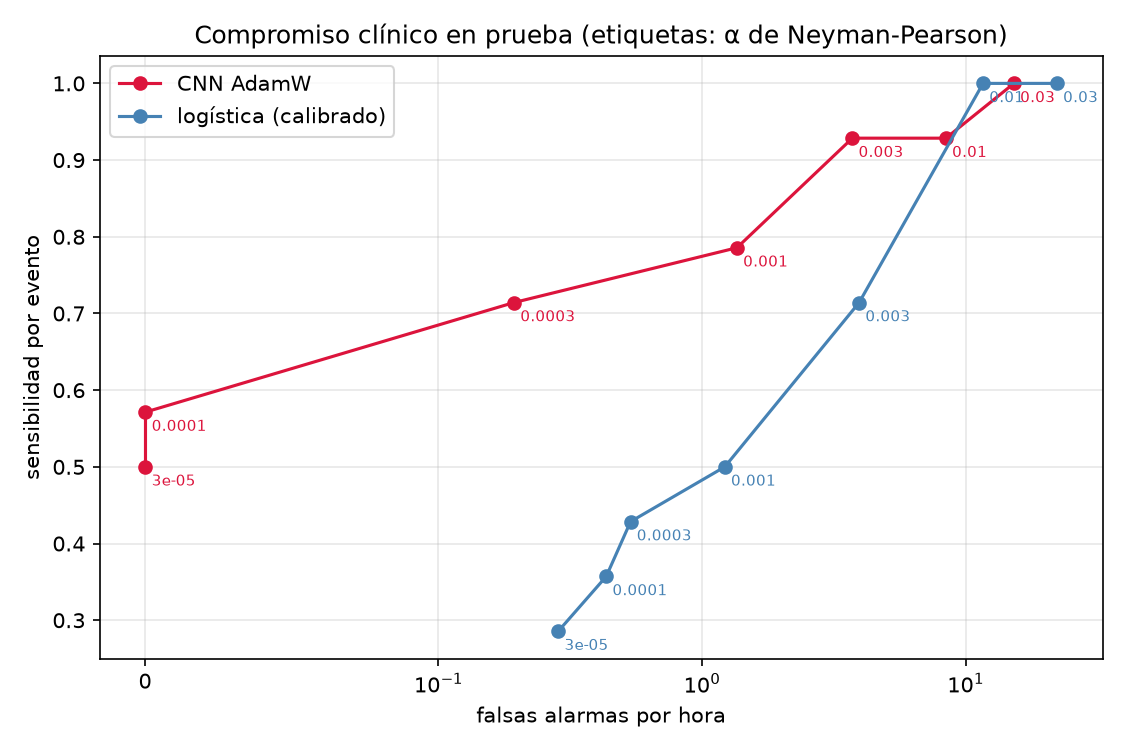
\includegraphics[width=0.8\textwidth]{etapa4/sensibilidad_vs_falsas_alarmas.png}
  \caption{Sensibilidad por evento contra falsas alarmas por hora en prueba, variando $\alpha$ (etiquetas). Eje horizontal
           lineal cerca de cero y logarítmico por encima de 0,1.}
  \label{fig:sens_fa}
\end{figure}

La Tabla~\ref{tab:barrido_alfa} y la Figura~\ref{fig:sens_fa} muestran:
\begin{itemize}
  \item \textbf{La CNN domina a la logística en toda la zona de pocas falsas alarmas.} Con $\alpha = 10^{-4}$ detecta 8 de 14
        crisis sin ninguna falsa alarma en 88 horas; con $\alpha = 3\times10^{-4}$, 10 de 14 con 0,19 falsas alarmas por hora
        (una cada 5 horas). La logística, para detectar 6 de 14, ya da 0,54 por hora.
  \item \textbf{La CNN también avisa antes}, para cualquier $\alpha$ a partir de $3\times10^{-4}$.
  \item \textbf{El compromiso es el que predice Neyman-Pearson}: al aflojar la restricción sube la sensibilidad y suben las
        falsas alarmas. El multiplicador $\lambda = dP_D/dP_{FA}$ se ve en la pendiente de la curva: entre $\alpha = 10^{-4}$ y
        $3\times10^{-4}$, la CNN gana 2 crisis por 0,19 falsas alarmas por hora; entre $10^{-2}$ y $3\times10^{-2}$, gana 1 crisis
        por 7 falsas alarmas por hora. Los rendimientos son decrecientes, como corresponde a una curva cóncava.
  \item \textbf{Detectar el 100~\% de las crisis es inaceptable con ambos modelos}: 15 falsas alarmas por hora con la CNN y 12
        con la logística.
  \item Con $\alpha \ge 10^{-2}$ la logística alcanza a la CNN en sensibilidad: las tres crisis que la CNN puntúa bajo sí las
        detecta la logística, pero solo cuando el umbral ya es muy permisivo.
\end{itemize}

Un punto de operación razonable para un monitor en una unidad de epilepsia sería $\alpha = 3\times10^{-4}$: 71~\% de las crisis
detectadas, con latencia mediana de 20~s y una falsa alarma cada 5 horas. Hay que tener presente que esos números salen de dos
pacientes y 14 crisis.

\section{Síntesis}
\label{sec:res_sintesis}

\begin{enumerate}
  \item Con la tasa elegida por validación, SGD supera significativamente a Momentum, Nesterov, Adam y AdamW
        ($p = 0{,}008$ en los cuatro casos), y no se distingue de RMSprop.
  \item Esa ventaja se explica casi por completo por la tasa de aprendizaje: en el experimento exploratorio con la tasa más
        alta de cada grilla, SGD, RMSprop, Adam y AdamW quedan empatados entre 0,970 y 0,976.
  \item La validación con un solo paciente está saturada (AUC de 0,996 a 0,999) y no predice la prueba ($\rho = -0{,}30$). Es la
        principal debilidad del diseño.
  \item Las diferencias en prueba se concentran en tres crisis de chb03; las otras 11 las reconocen todas las corridas.
  \item El modelo elegido, una de las peores corridas, detecta 11 de 14 crisis con 1,36 falsas alarmas por hora y 11~s de
        latencia, frente a 7 de 14, 1,22 y 26~s de la regresión logística calibrada, a pesar de tener menor AUC.
  \item El AUC no es la métrica adecuada para elegir un detector de crisis: lo que importa es la zona de $\text{FPR} \lesssim 10^{-3}$.
\end{enumerate}
